% @Author: YangZhou
% @Date:   2017-06-20 20:27:38
% @Last Modified by:   YangZhou
% @Last Modified time: 2018-01-10 23:52:08

\documentclass[aps,prb,twocolumn,showpacs,amsmath,amssymb]{revtex4-1}

\preprint{APS/123-QED}

\usepackage{graphicx}% Include figure filesxx
\usepackage{bm}% bold math
\usepackage{dcolumn}% Align table columns on decimal point
\usepackage{bm}% bold math

\usepackage{multirow}
\usepackage{epsfig}
\usepackage{amssymb}

\newcommand{\angstrom}{\mbox{\normalfont\AA}}

\begin{document}

\title{Anisotropic in-plane thermal conductivity in multilayer silicene}
\author{Yang Zhou${}^{1,3}$}
\author{Zhi-Xin Guo${}^{2,1}$}
\email{zxguo08@hotmail.com}
\author{Shi-You Chen${}^{1}$}
\author{Hong-Jun Xiang${}^{1}$}
\author{Xin-Gao Gong${}^{1,3}$}
\email{xggong@fudan.edu.cn}
\affiliation{
  ${}^1$Key Laboratory for Computational Physical Science (Ministry of Education), State Key Laboratory of Surface Physics and Department of Physics, Fudan University, Shanghai 200433, China\\
  ${}^2$Department of Physics, Xiangtan University, Xiangtan 411105, China\\
  ${}^3$Collaborative Innovation Center of Advanced Microstructures, Nanjing 210093, Jiangsu, China
}
\begin{abstract}
  We systematically study thermal conductivity of multilayer silicene by means of Boltzmann Transportation Equation (BTE) method.  We find that their thermal conductivity strongly depends on the surface structures. Thermal conductivity of bilayer silicene varies from $3.31$ W/mK to $57.9$ W/mK with different surface structures. Also, the $2\times1$ surface reconstruction induces unusual large thermal conductivity anisotropy, which reaches 70\%  in a four-layer silicene.  We also find that the anisotropy decreases with silicene thickness increasing, owing to the significant reduction of thermal conductivity in the zigzag direction and its slight increment  in the armchair direction.
  Finally, we find that both the phonon-lifetime anisotropy and the phonon-group-velocity  anisotropy contribute to the thermal conductivity anisotropy of multilayer silicene.
  These findings could be helpful in the field of heat management, thermoelectric applications involving silicene and other multilayer nanomaterials  with surface reconstructions in the future.

  \begin{description}
    \item[Keywords]
          Thermal conductivity, multilayer silicene, surface reconstruction, anisotropy
  \end{description}
\end{abstract}

\maketitle

\section{INTRODUCTION}

Many theoretical and experimental results showed that the quantum confinement and surface effects can remarkably reduce the thermal conductivity of nanomaterials while maintaining their electronic conductivity at high level, which make them great potential applications in the thermoelectric\cite{Dresselhaus2007,Chen2013}. For example,  Boukai \emph{et al}.\cite{Boukai2008} found that by altering the nanowire size and impurity doping levels,  approximately 100-fold improvement of  ZT over bulk Si can be achieved in a broad temperature range. Also, Hochbaum \emph{et al}.\cite{Hochbaum2008}  proposed a way of increasing ZT via controlling the roughness of silicene nanowires.
The combined effects of quantum size and surface reconstruction in multilayer silicene are expected to induce exotic thermal transport properties different from either monolayer silicene or bulk Si, which may make it suitable for the thermoelectric applications. Since thermal conductivity of monolayer silicene and bulk Si had been well explored, the investigation on multilayer silicene is helpful for understanding thermal conductivity evolution from two dimensional (2D) to three dimensional (3D) systems.

The existing researches on thermal conductivity of 2D materials mainly focus on the ones with weak van der Waals (vdW) interlayer interactions where no surface reconstruction appears. The multilayer graphene\cite{Lindsay2011, Ni2012,Wang2011}, $MoS_2$\cite{Liu2015}, and black phosphorus\cite{Zhang2015,Peng2015,Jain2015} are such kind of 2D materials which had been well studied.  Whereas, the thermal conductivity of 2D materials with strong interlayer interactions is poorly understood so far.
The multilayer silicene, which has been both theoretically predicted and experimentally synthesized, can be an ideal material for such an investigation \cite{Fu2014,Padova2016,Guo2015Structural}.The silicon materials present complex surface reconstructions, which are usually neglected for thermal conductivity investigations due to their small specific surface area. However, the reconstruction effect can be significant when a material's thickness becomes ultra thin, i. e., multilayer silicene.  Previous studies showed that multilayer silicene exhibits special surface reconstructions which induce  intriguing electronic property\cite{Fu2014,Guo2015Structural}. Naturally, one also expects the surface reconstruction to play a key role in its thermal transport property.

On the other hand, both experimental and theoretical studies showed that surface reconstruction in 2D materials can induce large anisotropy. For example, black phosphorus and phosphorene exhibit distinct thermal transport anisotropy owning to their puckered structures\cite{Zhang2015,Peng2015}.
The thermal transport anisotropy is closely relevant to the thermomechanical reliability of functional devices in nanoelectronics. In particular, alternative flexible substrate and active layer materials with increased thermal conductivity are  desirable  to prevent thermomechanical failures which have become a big challenge in flexible devices based on 2D materials\cite{Akinwande2014,Sadeghi2016}. Revealing the surface reconstruction effect on thermal conductivity anisotropy of multilayer silicene could stimulate the studies of covalently bonded 2D materials for the potential applications in the nanoelectronics.



\section{COMPUTATIONAL DETAILS}

The thermal conductivity of multilayer silicene structures are studied with the BTE method realized in ShengBTE\cite{Li2014}. In order to save the computing expense, the latest classical Mod potential\cite{Parks2007} implemented on the large scale parallel  molecular dynamics software package (LAMMPS) is chosen\cite{Kumagai2007Development}. This potential is able to reconstruct the elastic constant, melting point and phase transition of silicon materials. The potential parameters have been constructed for different type of silicene structures by fitting its bond angles to give accurate melting point and elastic constants, and for bulk Si with experimental equilibrium bond lengths which leads to smaller binding energy than that predicted by the first-principles calculations.

The atomic structures of multilayer silicene that were predicted to be stable by Guo \emph{et al}\cite{Guo2015Structural} are shown in Fig.\ref{fig:structures}. For convenience, we define the names of these structures as "nlxs", where "n" is a pure number, representing the number of layers, "l" means layer, "x" distinguishes different structures (concrete 1, 2, 3 etc. ) and "s"="a" or "z", corresponds to the silicene edge along the length direction, i. e.,  "a" for armchair) and "z" for zigzag. We also show in TABLE.\ref{tab:table1} the structure names and  minimum repeat cell periodicities of these multilayer silicene.


\begin{figure}[b]
  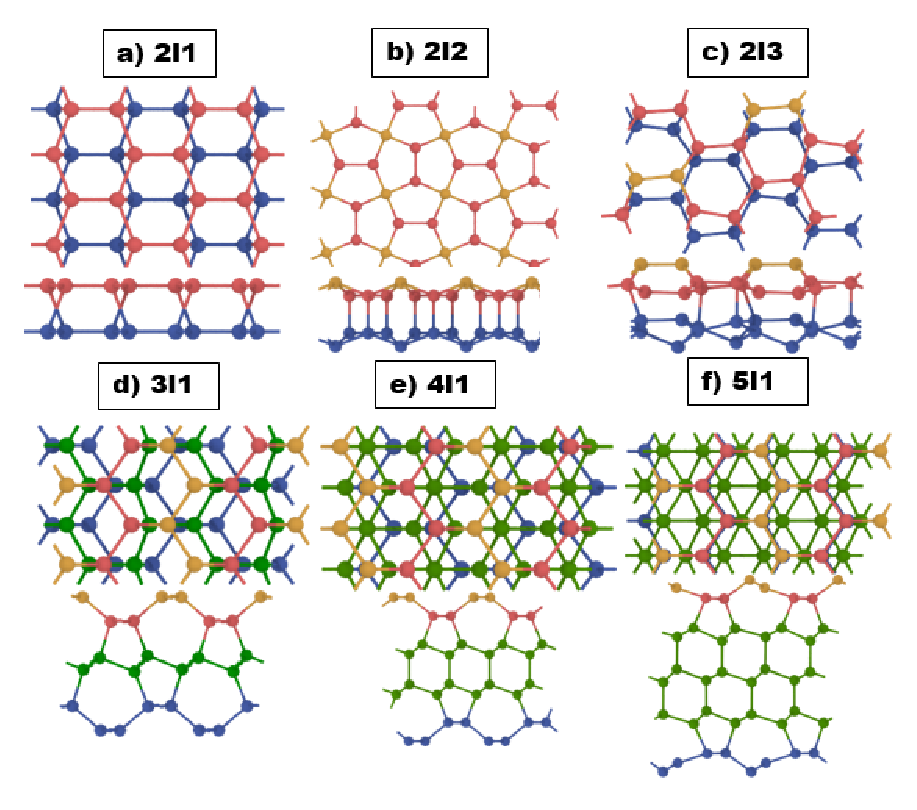
\includegraphics[angle= 0, width=0.95\linewidth]{images/structures.eps}
  \caption{\label{fig:structures}  (color online)  Top view and side views of typical structures of multilayer silicene. The buckling Si atoms on the top layer are labeled as yellow balls, and the red balls represent the remaining Si atoms on the top layer. All the Si atoms on the bottom layer are labeled as the blue balls. The green balls represent Si atoms in the middle layers. The orientation of top view of the cells is armchair in the x direction and zigzag in the y direction in the figure. The structures exihibit obvious and pretty different surface reconsruction.}
\end{figure}

Silicene structures are fully optimized using the conjugate gradient method.  The finite displacement method (FDM) realized in Phonopy\cite{Togo2008} and Thirdorder \cite{Li2014} are applied to extract the second- and third-order force constants (FCs) respectively,  in which hundreds of  slightly displaced supercells are generated. The obtained forces are calculated and used to calculate the FCs with the numerical differential calculation. The supercells of $3 \times 3 \times 1$ primitive cells are adopted to make the in-plane dimension above 40 \angstrom, which ensure the accuracy of calculated forces. Following the previous studies\cite{Pei2013,Fu2014}, we choose Si (111) layer spacing of $3.14 \angstrom$ as the interlayer thickness d because the thickness of two dimensional silicene is hard to restrictly determined, since it's a common constant for all the structures, the conclusion is independent on the absolute value of d, so a experimental value makes sence here.

The thermal conductivity tensor can be calculated as
\begin{equation}
  \kappa^{\alpha\beta} = \sum_{k \sigma}{c_{k \sigma}v^{\alpha}_{k \sigma}v^{\beta}_{k \sigma}\tau_{k \sigma}} \label{eq:kappasum}
\end{equation}
where $c_{k \sigma}$ is the heat capacity of phonon mode,  $v_{k \sigma}^{\alpha}$ is the mode group velocity, and $\tau_{k \sigma}$ is the phonon lifetime. The heat capacity is calculated by
\begin{equation}
  c_{k \sigma}=\frac{\hbar \omega_{k \sigma} }{V} \frac{\partial f(\omega_{k \sigma},T)}{\partial T} \label{eq:cv}
\end{equation}
where $ f(\omega,T)=1/[exp(\frac{\hbar \omega}{k_b T})-1]$ is the Bose-Einstein distribution function.

The calculations of $c_{k\sigma}$ , $v_{k \sigma}^{\alpha}$, and $\tau_{k\sigma}$ require the second- and third-order FCs as inputs, where the detailed formulas are referred to the work of  Li \cite{Li2014}. To avoid underestimation of thermal conductivity, the iteration method is used instead of the relaxation time approximation (RTA). A $45\times 45 \times 1$ Monkhorst-Pack q-point mesh is adopted for the convergence on the summation.

\section{RESULTS AND DISCCUSION}

We first show that the surface reconstruction has substantial influence on thermal conductivity of multilayer silicene.
Fig.\ref{fig:tc_length_sheng}(a) presents the length dependence of thermal conductivity of three structures of bilayer silicene.
One can see that the thermal conductivity converges quickly with cutoff phonon mean free path (MFP) in of 2l2 structure, while it is a bit slowly in 2l1 and 2l3 structures. Also, the cutoff MFPs of 2l1 structure are distinct in the armchair and zigzag directions. These features can be attributed to the different scattering intensity caused by the surface reconstructions.
It is known that the ballistic phonon transport is dominating when the length of the sample is smaller than the MFP,  whereas the diffuse phonon transport is  dominating when the length is larger than the MFP.
An empirical formula had been proposed by Thomas\cite{Thomas2010}  to characterize the thermal conductivity from ballistic to diffuse phonon-transport region, which is
\begin{equation}
  \kappa = \kappa_\infty (1-e^{-\frac{L}{L_c}}) \label{eq:eq_nemd}
\end{equation}
where $\kappa_\infty$ is the fitted full scattering thermal conductivity, $L_c$ is the transition length from the ballistic transportation to the diffuse transportation. Here we find that the length dependence of thermal conductivity of multilayer silicene can also be well described by such formula.
The saturated thermal conductivity of 2l1 structure reaches up to 42.1 (57.9) W/mK, while it is  31.1 (31.1) W/mK  for 2l2 structure and  3.3 (5.6)  W/mK for 2l3 structure in zigzag (armchair) direction, respectively,  showing the significant influence of surface reconstruction on thermal conductivity.

The surface reconstruction also induces thermal conductivity anisotropy, which can be evaluated using
\begin{equation}
  \chi=\frac{|\kappa_{z,\infty}-\kappa_{a,\infty} |}{ max⁡(\kappa_{z,\infty}-\kappa_{a,\infty} ) } \times 100 \%  \label{eq:eq_chi}
\end{equation}
with $ \kappa_{z,\infty} (\kappa_{a,\infty})$ being the full scattering thermal conductivity (infinite thermal conductivity) in the zigzag (armchair) direction.
It is found that both 2l2 and 2l3 structures show large thermal conductivity anisotropy, i.e., 27\% and 41\%, respectively, while 2l2 structure does not exhibits the anisotropy owning to its rotational symmetry over $\pi/2$.  The ultra-low and particularly high thermal conductivity anisotropy of bilayer silicene indicate its potential applications in the nanoelectronics.

\begin{figure}[b]
  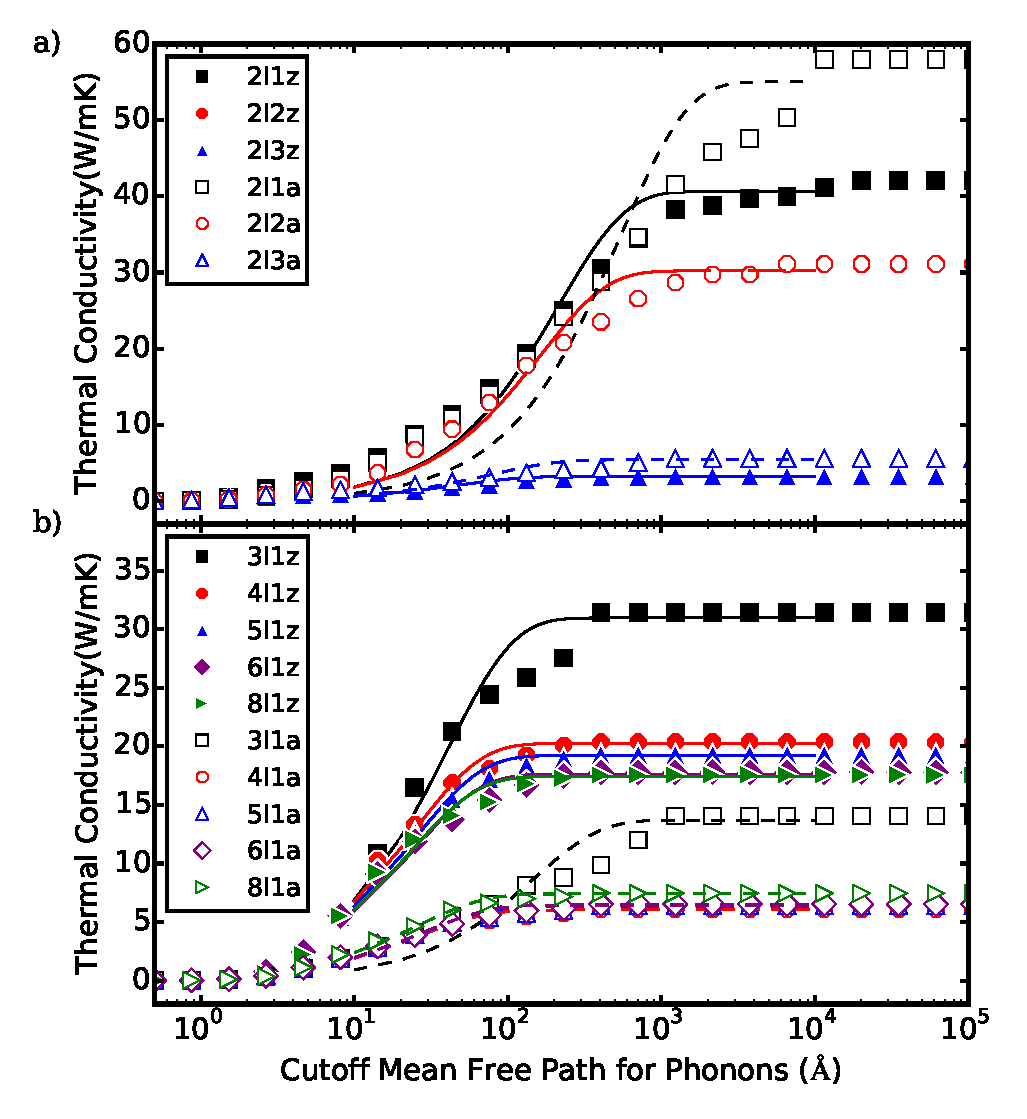
\includegraphics[angle= 0, width=0.9\linewidth]{images/tc_length_sheng.eps}
  \caption{\label{fig:tc_length_sheng} (color online) The depencence of cummulative thermal conductivity(TC) on cutoff phonon mean free path for all the structures. a) The cummulative TC of bilayer silicene structures. b) The cummulative TC of multilayer silicene with $2\times 1$ reconstruction and different layer. The dots are the results from BTE calculations, and the lines are the fitted results using Eq.(\ref{eq:eq_nemd}). The letter z/a in the legend means that the transport direction is zigzag/armchair. The dots of 2l2a and 2l2z are almost the same so red solid dots are covered. With the increase of cutoff mean free path TC converges. For bilayer structures TC along armchair direction is larger while for the others TC along zigzag direction is larger. With the increase of thickness TC along zigzag decreases while that along armchair increases a little. }
\end{figure}

\begin{figure}[b]
  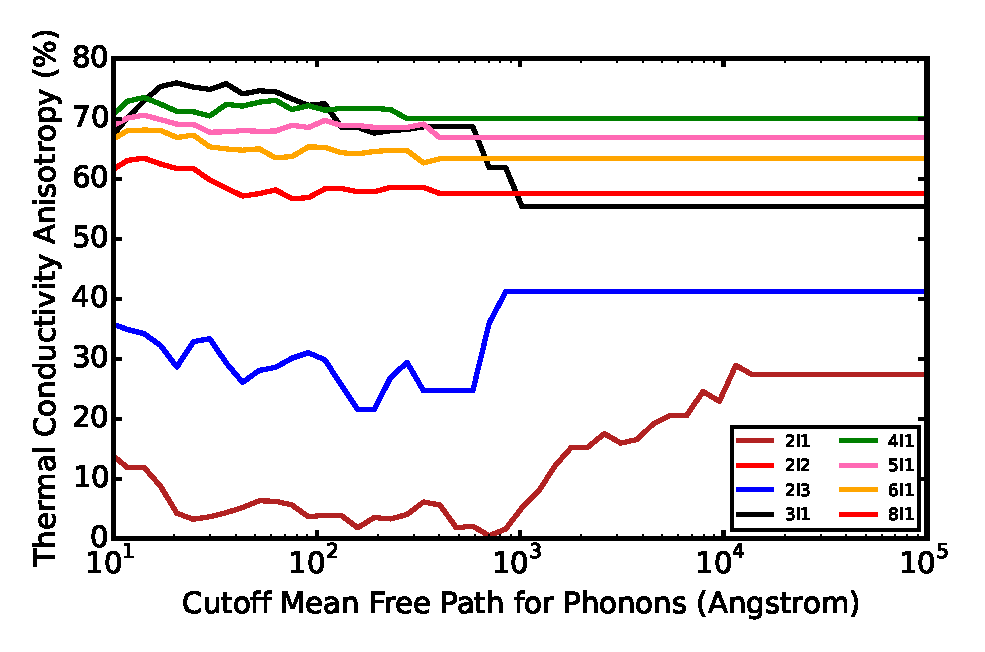
\includegraphics[angle= 0, width=0.9\linewidth]{images/chi.eps}{}
  \caption{\label{fig:chi} (color online) The dependence on cutoff MPF of cummulative TC anisotropy $\chi$. $\chi$ of 2l2 structure is exactly zero and is a horizonal line at 0. For 2l1, 2l3  structures the anisotropy increase with the cutoff MPF while that of 3l1 decreases. The others show indepencece of cutoff MPF. For bilayer silicence the anisotropy comes from long wave phonons while for multilayer structure it comes from phonons of all the wave length. }
\end{figure}

Here we discuss the thickness dependence of thermal conductivity anisotropy in multilayer silicene. We mainly focus on the structures of 3-8 Si layers in thickness, whose surface present the typical $2 \times 1$ Si(111) reconstruction. A common feature is that the thermal conductivity in the zigzag direction ($\kappa_z$) is obviously higher than that  in the armchair ($\kappa_a$) direction, which induces anisotropy larger than 55\%.
The reason is that the surface in zigzag direction is composed of smooth zigzag atomic chains (as shown in Fig.\ref{fig:structures}), which are favorable for the heat transport. Whereas,  there are large geometry fluctuations in the armchair direction, which are unfavorable for the heat transport.
With the silicene thickness increasing from 4 to 8 atomic layers, the anisotropy monotonically decreases from 70\% to 58\%, showing the negative  effect of thickness on the thermal conductivity anisotropy, which  is owing to the decrease of $\kappa_z$ and increase of $\kappa_a$  with the  thickness increasing.
One exception is for the trilayer silicene, which has the largest thermal conductivity but the smallest  anisotropy compared to the thicker  $2\times1$ silicene structures.  This could be understood by the direct interaction between the top and bottom layers, as well as the absence of ideal honeycomb ring under the surface layers  for the thermal transport, which is different from the thicker ones\cite{Guo2015Structural}.

We have also investigated the size effect on the thermal conductivity anisotropy. As shown in Fig.\ref{fig:chi}, the thermal conductivity of  2l1 bilayer silicene is almost isotropic with length of 10-1000 \angstrom, and it becomes increasingly anisotropic for length  above 1000  \angstrom. This is essentially due to the difference of acoustic phonons in different directions,  which have large MFP.  As for the $2\times1$ structures with 3-8 Si layers in thickness, the high thermal conductivity anisotropy is obtained even when the length is as short as 10 \angstrom, implying that the anisotropy is  mainly induced by the optical phonons. On the other hand, the thermal conductivity anisotropy of 2l3 silicene can be owning to both acoustic and  optical phonons in different directions.

\begin{table*}
  \caption{\label{tab:table1}
    The thermal conductivity and its anisotropy of different multilayer silicene, along with the average heat capacity ($kJ/m^3/K$) of zigzag ( $Cv_z$) and armchair ($Cv_a$) directions, respectively. }
  \begin{ruledtabular}
    \begin{tabular}{ccccccc}
          & Minimal period
          & $\kappa_{z,\infty}$
          & $\kappa_{a,\infty}$
          & $\chi$
          & $Cv_{z}$
          & $Cv_{a}$                                                           \\
      \hline
      2l1 & $1 \times 1$             & 42.10 & 57.92 & 27.31\% & 165.8 & 166.7 \\
      2l2 & $\sqrt{2}\times\sqrt{2}$ & 31.11 & 31.11 & 0    \% & 38.44 & 38.44 \\
      2l3 & $2 \times 2$             & 3.311 & 5.624 & 41.13\% & 22.42 & 22.42 \\
      3l1 & $2 \times 1$             & 31.44 & 14.05 & 55.29\% & 52.22 & 52.46 \\
      4l1 & $2 \times 1$             & 20.37 & 6.114 & 69.98\% & 37.71 & 37.89 \\
      5l1 & $2 \times 1$             & 19.33 & 6.419 & 66.78\% & 29.17 & 29.32 \\
      6l1 & $2 \times 1$             & 17.78 & 6.527 & 63.29\% & 23.73 & 23.86 \\
      8l1 & $2 \times 1$             & 17.56 & 7.461 & 57.51\% & 17.26 & 17.36 \\
    \end{tabular}
  \end{ruledtabular}
\end{table*}

To explore the origin of thermal conductivity anisotropy, we have calculated the phonon frequency distributions of thermal conductivity in armchair and zigzag directions  (Fig.\ref{fig:tc_freq}).
It is found that the anisotropy is mainly attributed to the low-frequency (0-5 THz) phonons for the bilayer silicene, i. e., 2l1 and 2l3, where thermal conductivity in armchair direction is obviously larger than that in zigzag direction.
Whereas, as for the $2\times1$ structures thicker than 3 Si layers, the thermal conductivities in armchair and zigzag directions are nearly the same in the low-frequency region, and the anisotropy is mainly attributed to the high-frequency (5-20 THz) phonons.
In addition, the anisotropy of the 3l1 structure is resulted by the phonons with frequency above 10 THz, below which the summation of contributions to thermal conductivity are nearly the same in armchair and zigzag directions.

To have a deep insight into the origin of anisotropy, it's helpful to investigate all the factors that contribute to thermal conductivity according to Eq.(\ref{eq:kappasum}).
We select all the phonons along  $\Gamma\rightarrow X$ and $\Gamma \rightarrow Y$ directions in Brillouin zone, and calculated their heat capacity with Eq.(\ref{eq:cv}). The averaged heat capacity of silicene structures are shown in Table.\ref{tab:table1}, where $Cv_z$ and $Cv_a$ correspond to the  heat capacity for thermal conductivity in the zigzag and armchair directions, respectively.  As one can see, although $Cv_z$ and $Cv_a$  strongly depend on the reconstructed structure and thickness of multilayer silicene, their difference in the same structure is very small. This feature shows that the thermal conductivity anisotropy is insensitive to the heat capacity.


\begin{figure}[b]
  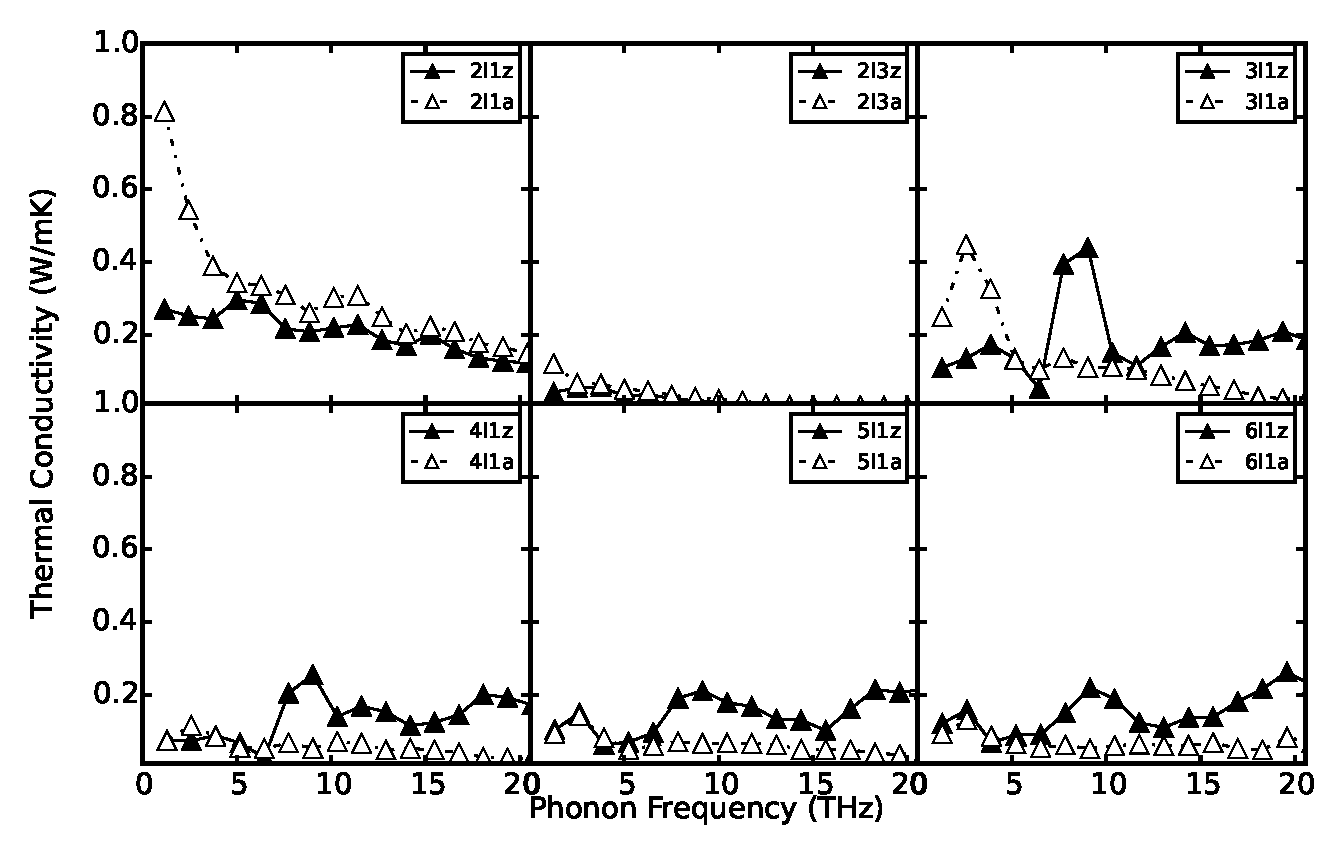
\includegraphics[width=1\linewidth]{images/tc_freq.eps}
  \caption{\label{fig:tc_freq} (color online)  The phonon frequency dependence of converged thermal conductivity of multilayer silicene. For bilayer structures TC mainly comes from low frequency phonons while the others have more contribution from high frequency phonons and they have similar curve. TC of bilayer structure have larger TC along armchair direction at low frequency and the anisotropy deceases with frequency. For the other structures, TC shows little difference along the two direction at low frequency but TC along zigzag direction is higher at high frequency. }
\end{figure}

\begin{figure}[b]
  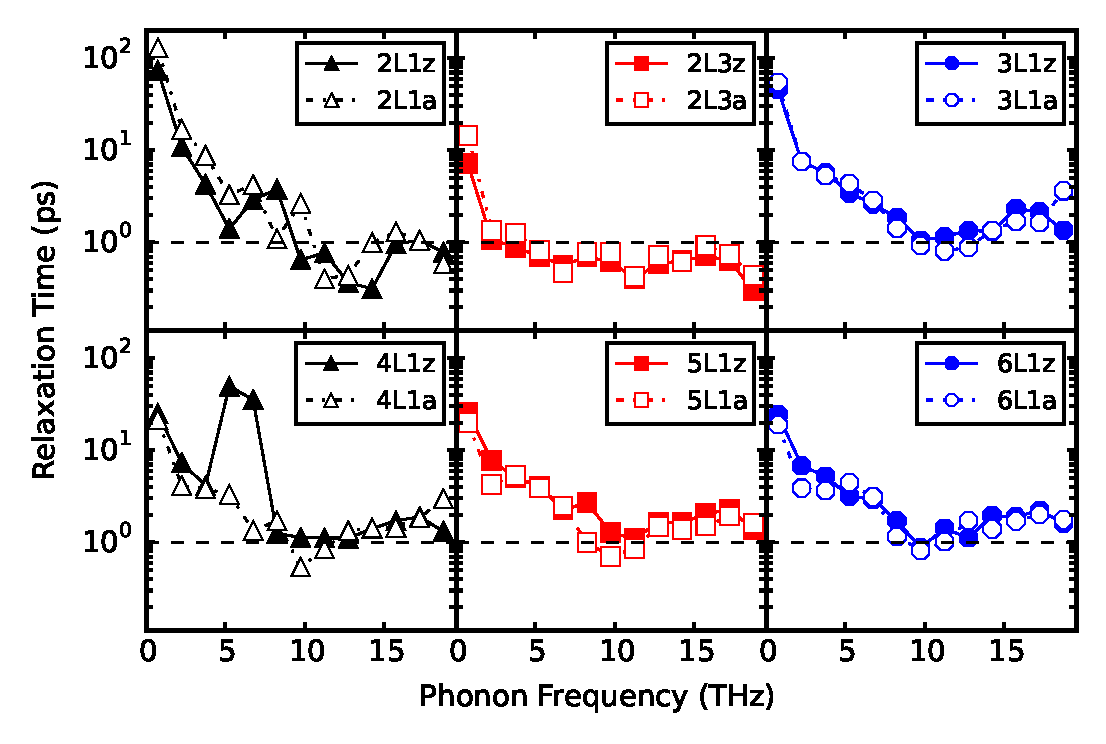
\includegraphics[width=1\linewidth]{images/tau.eps}
  \caption{\label{fig:tau} (color online)  Phonons lifetimes of multilayer silicene obtained by considering the three-phonon scattering process.  The horizonal dash line at 1.0ps is a guidence for the main contribution region of phonon frequency. Phonon lifetime doent's show obvious anisotropy in both bilayer structure and multilayer structures (except for the anmornal region of 5-7 THz in 4l1 structure). The main contribution of lifetime comes from low frequency phonons in bilayer structures while the others have relative uniform contribution from the frequency domain.  }
\end{figure}

\begin{figure}[b]
  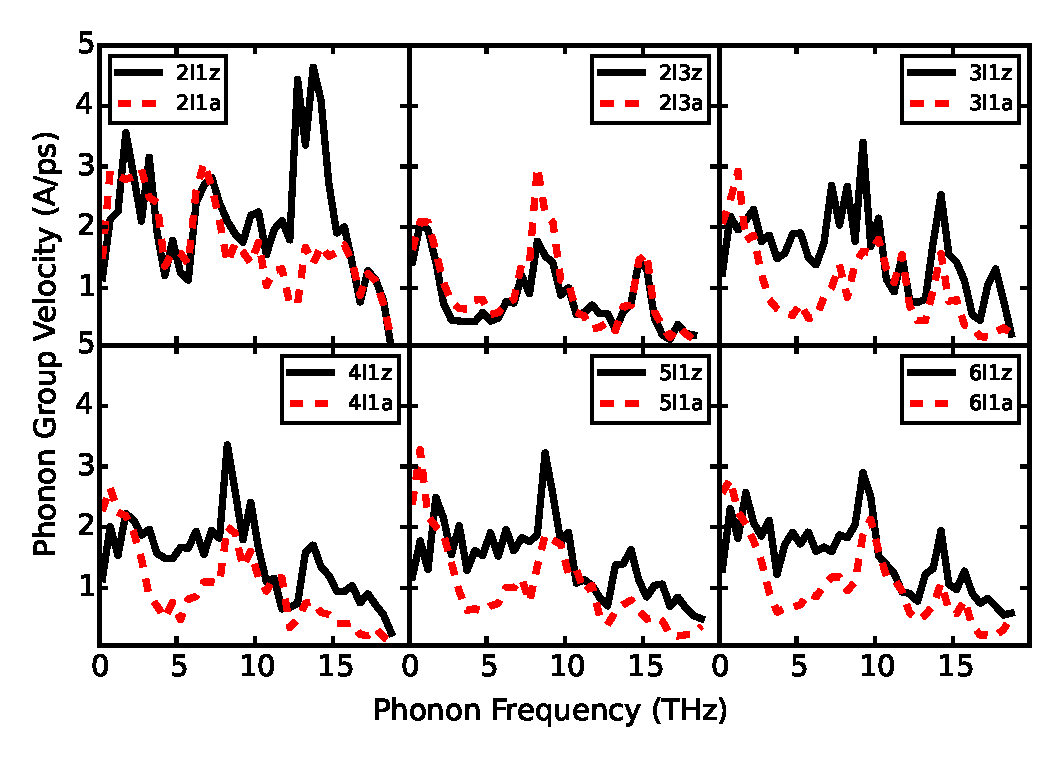
\includegraphics[width=0.9\linewidth]{images/gv.eps}{}
  \caption{\label{fig:gv} (color online) Group velocities versus phonon frequencies in both the zigzag and armchair directions of multilayer silicene. The histogram bin width is chosen as 1.5 THz. The bilayer structures have isotropic group velocities at low frequency region and the contribution from high frequency could be ignored considering the valishment of lifetime at this region. The structure of 3-6 layers exhibit anisotropic group velocity which suggests localization of phonons.}
\end{figure}
We then explore the contributions from the phonon lifetimes for the thermal conductivity anisotropy.
We have considered the three-phonon scattering process, where the scattering rate is obtained from the Fermi-golden's rule\cite{Li2014} under the relaxation time approximation (RTA). The iterative method was then adopted to include the cross influence of the phonon excitation, since it usually gives lager but more accurate lifetimes than the RTA. The frequency dependence of phonon lifetimes calculated with ShengBTE\cite{Li2014} are shown in Fig.\ref{fig:tau}, where the values are averaged for frequency bins to reduce complexity.  It is shown that the lifetimes of larger than 1 ps for bilayer silicene structures (2l1, 2l3) distribute on the low-frequency region, indicating the dominating contributions of low-frequency phonons to the thermal conductivity. Moreover, the lifetimes in armchair direction are obviously larger than that in zigzag direction in the low-frequency region. This feature indicates that the thermal conductivity anisotropy of bilayer silicene is attributed to the difference of phonon lifetimes in different directions.
On the other hand, the phonon lifetimes exhibit a different frequency distribution for the thicker silicene, i. e.,  $2\times1$ structures with 3-6 Si layer in thickness, where the phonon lifetimes larger than 1 ps cover both the low and high frequency regions.  This explains why the high frequency phonons contribute significantly to the thermal conductivity in the thicker silicene (Fig. \ref{fig:tc_freq}).  However, except for the 4l1 structure, the phonon lifetimes in zigzag and armchair directions are very close for the $2\times1$ structures, implying their tiny effect on the thermal conductivity anisotropy.



To further explore the origin of thermal conductivity anisotropy in multilayer silicene, we have calculated the frequency dependence of phonon group velocities in armchair and zigzag directions. As shown in Fig. \ref{fig:gv},  the group-velocity difference in the two directions is very small in the low-frequency region for the bilayer silicene. This result confirms that the thermal conductivity anisotropy mainly comes from the different phonon scatterings in the armchair and zigzag directions,  which induce different phonon lifetimes.
As for the $2\times 1$ silicene with thickness more than three Si layers,  the group velocity in zigzag direction is obviously larger than that in the armchair direction in most of the frequency region. Considering that the phonon-lifetime difference contributes little to the anisotropy for 3l1, 5l1, and 6l1 structures, one can conclude that the group velocity difference is the main reason for the thermal conductivity anisotropy of $2\times 1$ multilayer silicene. It should be noted that the anisotropy of 4l1 structure is from the contributions of both phonon lifetime and group velocity, which lead to its unusual large anisotropy up to 70\%.

\section{CONCLUSIONS}
By means of Boltzmann Transportation Equation methods, we have investigated the thermal conductivity of multilayer silicene with various surface structures and thicknesses.
We have found that the surface reconstruction has significant effect on the thermal conductivity of multilayer silicene.  The smooth surface is favorable for heat conduction, while the rough surface greatly suppresses the heat conduction. Both ultra-low (3.3 W/mK) and relatively high (57.9 W/mK) thermal conductivities have been obtained on bilayer silicene with different surface structures, which also induce large anisotropy of 41\% and 27\%, respectively. We have also found that the $2 \times 1$ surface reconstruction induces the unusual large thermal conductivity anisotropy of 70\%  in the four-layer silicene.  Moreover, we have found that increasing silicene thickness, which has an effect of weakening the surface contribution to the thermal transport, reduces the thermal conductivity anisotropy. Finally, we have clarified that the anisotropy from phonon lifetimes and phonon-group velocities contributes most to the thermal conductivity anisotropy to the bilayer and thicker $2\times 1$ silicene structures, respectively. Our results indicate that multilayer silicene with thickness of 2-4 layers present the most exotic physical properties, which may be a common feature for the 2D materials with strong interlayer interactions.
This work is expected to helpful in the field of heat management, thermoelectric applications involving silicene and other multilayer nanomaterials in the future.


\section{ACKNOWLEDGEMENTS}
This paper was partially supported by the National Natural Science Foundation of China, the Special Funds for Major State Basic Research, the Foundation for the Author of National Excellent Doctoral Dissertation of China, the Program for Professor of Special Appointment at Shanghai Institutions of Higher Learning, and the Research Program of Shanghai Municipality and the Ministry of Education.


\bibliography{ref}
\end{document}
